
\section{Evaluation}
\label{sec:evaluation}
To rigorously assess the performance of \approach{}, we evaluate \Blue{four} research questions:

\begin{itemize}
	\item \textbf{RQ1 (Effectiveness)}: How effectively does \approach{} perform relative to state-of-the-art methods in attack detection?
	\item \textbf{RQ2 (Ablation Study)}: How significantly do different components contribute to the system's performance?
	\item \textbf{RQ3 (Backbone Ablation)}: How does replacing the LLM backbone affect \approach{}\textquotesingle s detection performance?
	\item \textbf{RQ4 (Efficiency)}: How efficient are \approach{} in terms of computational resources and time?
\end{itemize}



\begin{figure*}[t]
	\centering
	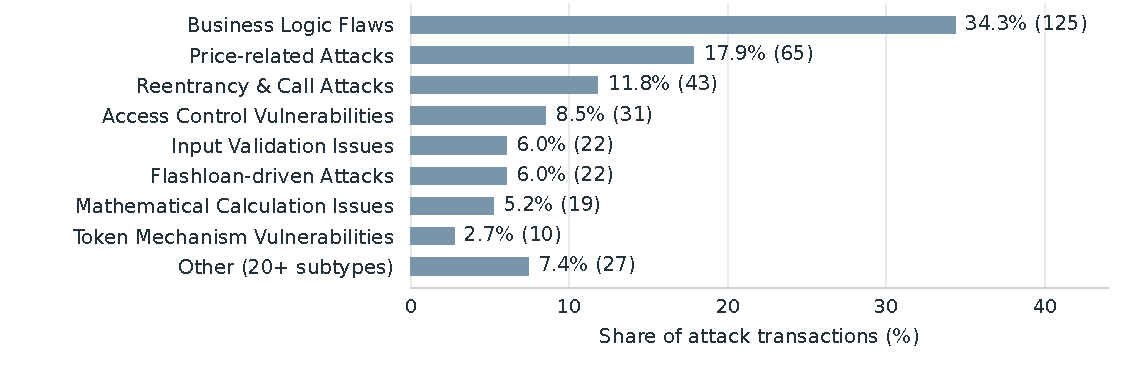
\includegraphics[width=\textwidth]{pic/attack_distribution_bar.pdf}
	\caption{\Blue{Distribution of the 364 attack transactions in \dsystem{}, drawn from DeFiHackLabs. Labels report the percentage and count for each category.}}
	\label{tab:attack_categories}
\end{figure*}

\textit{\textbf{\Blue{Datasets.}}}
\Blue{We use a transaction dataset constructed for this study and a price-manipulation dataset introduced by DeFiScope~\cite{zhong2025detectingvariousdefiprice}.}

\Blue{\textbf{\dsystem{}.} We construct this evaluation set from 364 attack transactions drawn from DeFiHackLabs~\cite{defihacklabs2024}, a public repository of real-world exploit reproductions, and 364 benign transactions sampled from normal user activity in the affected protocols. The benign transactions are selected using temporal proximity to the attacks. We call the resulting balanced set of 728 transactions \dsystem{}. The attack cases span January 2021 to January 2025 and include 110+ labeled exploit types across blockchains such as Ethereum, BSC, and Arbitrum.}
\textcolor{red}{We randomly shuffle the overall transaction collection before partitioning it for model training, knowledge-base construction, and evaluation. The 728 test transactions are disjoint from both the transactions used to train XGBoost and those used to construct the RAG knowledge base.}
\Cref{tab:attack_categories} shows the attack distribution and their proportions.
Business logic flaws and price-related attacks are the most common, accounting for 34.3\% and 17.9\% of the dataset, respectively. Reentrancy and call attacks, access control vulnerabilities, input validation issues, flashloan-driven attacks, mathematical calculation issues, token mechanism vulnerabilities, and other miscellaneous attack types make up the remaining 47.8\%.

\Blue{\textbf{\done{}.} We use the D1 dataset introduced by DeFiScope~\cite{zhong2025detectingvariousdefiprice} for price-manipulation detection. DeFiScope assembled its 95 real-world attacks from DeFort, DeFiHackLabs, and its industry partner, removing duplicate cases across these sources. The attacks caused a reported total loss of \$381.16M on Ethereum and BSC. We could not parse transaction data for four cases and evaluate the remaining 91 attack transactions. We denote this evaluated subset \done{} throughout the paper.}

\textit{\textbf{Baselines.}}
To the best of our knowledge, TrxGNNBERT~\cite{TrxGNNBERT}, TxSpector~\cite{TXSPECTOR}, Blockscan~\cite{wu2025blockscan}, DeFiScope~\cite{zhong2025detectingvariousdefiprice}, DeFort~\cite{defort2024}, DeFiRanger~\cite{defiranger2021}, and DeFiTainter~\cite{defitainter2023} are the most relevant and representative baselines for our evaluation.
Particularly,  TrxGNNBERT~\cite{TrxGNNBERT} powered by a Graph-Transformer architecture, TxSpector~\cite{TXSPECTOR} leveraging static opcode analysis, and Blockscan~\cite{wu2025blockscan} using BERT model enhanced with masked language modeling mechanism, are evaluated on \dsystem{} dataset.
For specialized price manipulation detectors, DeFiScope~\cite{zhong2025detectingvariousdefiprice} combining fine-tuning and pattern learning, DeFort~\cite{defort2024} harnessing symbolic execution and runtime monitoring, and DeFiRanger~\cite{defiranger2021}, and DeFiTainter~\cite{defitainter2023} based on a inter-contract taint analysis, are evaluated on \done{} dataset.
\textcolor{red}{XGBoost-only directly classifies transactions from numerical features. In \approach{}, XGBoost instead guides context selection and prompting, with the LLM producing the final classification. This baseline comparison evaluates direct numerical classification against the combined pipeline.}


\textit{\textbf{Experiment Setup.}}
\Blue{LLMs are accessed through third-party APIs. We implement the pipeline with LangChain~\cite{langchain}, Chroma~\cite{chromadb}, and Jina Embeddings v3~\cite{jina2024}. We evaluate nine LLM backbones using the complete pipeline in Figure~\ref{fig:flowchart}; RQ3 compares their detection performance. We treat attacks as the positive class and report accuracy, precision, recall, and F1. For configurations with invalid outputs, metrics are computed on valid predictions and accompanied by prediction coverage.}

\Blue{The XGBoost-only baseline uses 420 training samples and 728 test samples, with balanced attack and benign classes in each set. The tree settings are maximum depth 3, learning rate 0.02, and minimum child weight 1. Row and column subsampling ratios are 0.9 and 0.7; $L_1$ and $L_2$ regularization coefficients are 0 and 0.5.}

\textcolor{red}{We selected the parameter settings empirically based on detection performance in preliminary trials. The LLM prompt includes the XGBoost attack probability as an auxiliary risk signal, using 0.5 as the reference threshold. A probability below 0.5 prompts closer scrutiny of potential false positives; the LLM makes the final decision based on transaction evidence.}






\subsection{RQ1 (Effectiveness): Comparative Analysis of Detection Accuracy}
To provide a comprehensive assessment of \approach{}'s detection efficacy, we conducted comparative experiments across two datasets with distinct characteristics.
\Blue{\approach{} reduces false alarms while maintaining recall close to XGBoost-only (\Cref{tab:performance-dsystem-compact}). It correctly classifies 679 of 728 transactions and achieves 92.93\% F1, compared with 86.48\% for XGBoost-only. Precision rises from 84.33\% to 97.87\%, and false positives fall by 88.33\% (60 to 7), with one additional false negative (41 to 42). XGBoost-only achieves a test AUC of 0.9467. Comparisons with the external baselines are descriptive because their evaluation coverage and class composition differ.}

\Blue{The external baselines show different detection trade-offs. Blockscan achieves 95.5\% precision but 70.1\% recall, missing 109 attacks; its F1 is 81.0\%. TrxGNNBERT reports 76.6\% F1, while TxSpector achieves 53.3\% F1 on the 450 transactions it processes. \approach{} combines 97.87\% precision with 88.46\% recall. Relative to Blockscan, this balance corresponds to both fewer false positives (7 versus 12) and fewer missed attacks (42 versus 109).}



\begin{table}[t]
\centering\color{blue}\small
\caption{\Blue{Detection performance on \dsystem{}. \approach{} and XGBoost-only use 364 attack and 364 benign samples. Metrics are percentages.}}
\label{tab:performance-dsystem-compact}
\setlength{\tabcolsep}{2pt}
\begin{tabular}{@{}lrrrrr@{}}
\toprule
Metric & TxSpector & \makecell{TrxGNN\\BERT} & Blockscan & \makecell{XGBoost-\\only} & \approach{}\\
\midrule
$N$ &450&728&728&728&728\\
TP &117&288&255&323&322\\
FP &117&91&12&60&7\\
TN &128&264&352&304&357\\
FN &88&85&109&41&42\\
\midrule
Acc. &54.4&75.9&83.4&86.13&93.27\\
Prec. &50.0&76.0&95.5&84.33&97.87\\
Rec. &57.1&77.3&70.1&88.74&88.46\\
F1 &53.3&76.6&81.0&86.48&92.93\\
\bottomrule
\end{tabular}
\smallskip\par\footnotesize
$N$ denotes the number of evaluated transactions. TxSpector processes 450 of 728 transactions; EVM instruction support and runtime limitations prevent completion on the remaining 278. Its metrics are computed on the 450 processed transactions. The TrxGNNBERT counts correspond to 373 attacks and 355 benign samples, rather than 364/364; its metrics are reported on that class composition. Runtime is analyzed separately in RQ4.
\end{table}




\begin{table}[t]
	\centering
	\caption{\Blue{Detection performance on \done{}, the 91-attack subset of DeFiScope\textquotesingle s D1 dataset~\cite{zhong2025detectingvariousdefiprice}.}}
	\label{tab:recall-d1-dataset}
	\small
\setlength{\tabcolsep}{4pt}
	\begin{tabular}{l c c c}
		\toprule
		\text{Tool} &
		\text{\#Attack} &
		\text{Detection Rate} &
		\text{$\Delta$Detection Rate} \\
		\midrule
		DeFort (DF)             & 50  & 54.95\% & $-$25.27\% \\
		DeFiRanger (DR)         & 48  & 52.75\% & $-$27.47\% \\
		DeFiTainter (DT)        & 32  & 35.16\% & $-$45.06\% \\
		DeFiScope (DS)          & 73  & 80.22\% & \textbf{Baseline} \\
		\approach{}   & 86 & 94.51\% & +14.29\% \\
		\bottomrule
	\end{tabular}
\end{table}
\Blue{On \done{}, \approach{} detects 86 of 91 attacks, achieving 94.51\% recall compared with 80.22\% for DeFiScope (Table~\ref{tab:recall-d1-dataset}). The \done{} experiment evaluates specialized price-manipulation detection separately from the \dsystem{} experiment. Table~\ref{tab:ragflow_false_negative} lists the five missed cases.}




\begin{table}[t]
	\centering
	\caption{\Blue{Missed price-manipulation attacks and baselines' detection results.}}
	\label{tab:ragflow_false_negative}
	\small
	\begin{tabular}{l c c c c}
		\toprule
		Attack Case & DS & DT & DF & DR \\
		\midrule
		MerlinLab & \ding{51} & \ding{55} & \ding{55} & \ding{55} \\
		BeltFinance\_1 & \ding{51} & \ding{51} & \ding{55} & \ding{51} \\
		BeltFinance\_2 & \ding{51} & \ding{51} & \ding{55} & \ding{51} \\
		IndexedFinance & \ding{55} & \ding{55} & \ding{55} & \ding{51} \\
		ERC20TokenBank & \ding{51} & \ding{55} & \ding{55} & \ding{51} \\
		\bottomrule
	\end{tabular}
	
	\vspace{0.3em}
	\footnotesize\textit{DS=DeFiScope, DT=DeFiTainter, DF=DeFort, DR=DeFiRanger. \ding{51}=detected, \ding{55}=missed.}
\end{table}

\Blue{The five missed price-manipulation attacks expose challenges in recognizing protocol-specific economic logic and multi-step interactions.}

A deep dive into these misjudgments reveals that \approach{}’s limitations are primarily confined to four scenarios. First are rare or highly customized oracle manipulation patterns (e.g., MerlinLab), which exploit idiosyncratic oracle update windows; the absence of sufficiently similar historical samples causes analogical reasoning to falter. Second, the system struggles with arbitrage attacks involving complex multi-step cross-contract interactions (e.g., BeltFinance), where attackers leverage minute price discrepancies through sequences of transactions that appear legitimate in isolation, making full-chain reconstruction difficult. Third, novel attacks utilizing innovative mechanisms (e.g., IndexedFinance), such as exploiting index token rebalancing weights, fall outside the scope of historical patterns or rule-based detection. Finally, atypical price manipulation edge cases (e.g., ERC20TokenBank) manipulate internal accounting logic rather than liquidity pool pricing, a paradigm shift that often leads to omissions by most detection tools.



\begin{tcolorbox}[colback=black!5!white,colframe=black!75!black,sharp corners,fontupper=\small,title=Answer to RQ1]
\Blue{\approach{} achieves 92.93\% F1 and 97.87\% precision. Compared with direct XGBoost classification, it reduces false positives from 60 to 7 with one additional false negative. On \done{}, recall reaches 94.51\%.}
\end{tcolorbox}

\subsection{\Blue{RQ2 (Ablation Study): Effects of Component Configurations}}
\Blue{We fix the default backbone and compare the complete system with three ablated configurations: without XGBoost, without both XGBoost and two-stage retrieval, and without RAG. \textcolor{red}{The no-XGBoost configuration removes numerical risk guidance from context selection and prompting.} The first two ablated configurations yield valid predictions for all 728 transactions. The no-RAG configuration yields 726 valid predictions; its two invalid outputs correspond to attacks.}

\begin{table*}[t]
\centering\color{blue}\small
\caption{\Blue{Component ablation results. Metrics are percentages on valid predictions; counts are ordered TP/FP/TN/FN.}}
\label{tab:ragflow-ablation}
\setlength{\tabcolsep}{3pt}
\begin{tabular}{lrlrrrr}
\toprule
Configuration & $N$ & TP/FP/TN/FN & Acc. & Prec. & Rec. & F1\\
\midrule
Full system &728&322/7/357/42&93.27&97.87&88.46&92.93\\
w/o XGBoost &728&295/98/266/69&77.06&75.06&81.04&77.94\\
w/o XGBoost + two-stage &728&315/110/254/49&78.16&74.12&86.54&79.85\\
w/o RAG &726&278/98/266/84&74.93&73.94&76.80&75.34\\
\bottomrule
\end{tabular}
\smallskip\par\footnotesize
\textcolor{red}{The w/o XGBoost + two-stage configuration removes both components. No-RAG coverage is 726/728 (99.73\%); two invalid outputs are excluded. Metrics compare predictions from the respective model configurations.}
\end{table*}

\Blue{\textbf{\textcolor{red}{XGBoost guidance.}} \textcolor{red}{The comparison measures the contribution of numerical risk guidance to context selection and prompting. These inputs affect the LLM decision, so removing XGBoost can change both false positives and false negatives.} Relative to the no-XGBoost variant, the complete system produces 91 fewer false positives and detects 27 more attacks. These differences correspond to gains of 14.99, 22.81, and 7.42 percentage points in F1, precision, and recall, respectively. \textcolor{red}{At the transaction level, the complete system correctly classifies 93 benign transactions and 39 attacks misclassified by the no-XGBoost variant, but misclassifies two benign transactions and 12 attacks correctly classified by that variant.}}

\Blue{\textbf{Two-stage retrieval.} \textcolor{red}{Without XGBoost, F1 is 77.94\% with two-stage retrieval and 79.85\% without it, a decrease of 1.91 percentage points when retrieval filtering is retained.} Its precision is slightly higher (75.06\% versus 74.12\%), but recall is lower (81.04\% versus 86.54\%). \textcolor{red}{The complete system exceeds the variant without both XGBoost and two-stage retrieval by 13.08 percentage points in F1.}}

\Blue{\textbf{No-RAG comparison.} On the 726 transactions with valid predictions in both configurations, the complete system achieves 92.89\% F1, compared with 75.34\% without RAG, a difference of 17.55 percentage points.}

\begin{tcolorbox}[colback=black!5!white,colframe=black!75!black,sharp corners,fontupper=\small,title=Answer to RQ2]
\Blue{The complete configuration improves F1 by 14.99 percentage points over the no-XGBoost configuration and by 17.55 percentage points over the no-RAG configuration on their shared valid samples. Without XGBoost, two-stage retrieval trades higher precision for lower recall and F1.}
\end{tcolorbox}

\begin{figure*}[t]
\centering
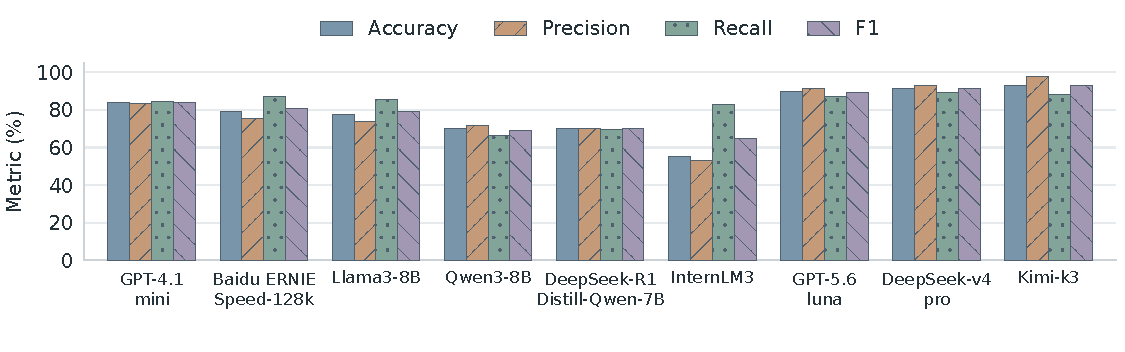
\includegraphics[width=\linewidth]{pic/model_performance_column_chart.pdf}
\caption{\Blue{Detection performance across nine LLM backbones on \dsystem{}. Metrics are percentages.}}
\label{tab:ragflow_results}
\label{fig:backbone_results}
\end{figure*}

\subsection{\Blue{RQ3 (Backbone Ablation): Choice of LLM Backbone}}

\Blue{Figure~\ref{fig:backbone_results} presents the backbone ablation, replacing the default LLM with eight alternatives while retaining the complete \approach{} pipeline. The default backbone achieves the highest precision and F1, with seven false positives, while DeepSeek-v4-pro detects the most attacks. DeepSeek-v4-pro detects 325 attacks compared with 322 for the default backbone, but produces 24 false positives. GPT-5.6-luna detects 318 attacks and produces 29 false positives. Table~\ref{tab:backbone_results} provides the confusion counts and metrics for the default backbone, DeepSeek-v4-pro, and GPT-5.6-luna.}

\Blue{The other backbones exhibit different precision--recall trade-offs within the same pipeline. GPT-4.1-mini achieves 83.9\% F1, with 83.2\% precision and 84.6\% recall. Baidu ERNIE-Speed-128k and Llama3-8B reach higher recall (87.1\% and 85.4\%), but lower precision (75.5\% and 74.1\%), yielding F1 scores of 80.9\% and 79.3\%, respectively.}



\begin{table}[t]
\centering\color{blue}\small
\caption{\Blue{Detailed results for three LLM backbones using the complete \approach{} pipeline ($N=728$ each). Metrics are percentages.}}
\label{tab:backbone_results}
\begin{tabular}{@{}lrrr@{}}
\toprule
Metric & Kimi-k3 & \makecell{DeepSeek-\\v4-pro} & \makecell{GPT-5.6-\\luna}\\
\midrule
TP &322&325&318\\
FP &7&24&29\\
TN &357&340&335\\
FN &42&39&46\\
\midrule
Acc. &93.27&91.35&89.70\\
Prec. &97.87&93.12&91.64\\
Rec. &88.46&89.29&87.36\\
F1 &92.93&91.16&89.45\\
\bottomrule
\end{tabular}
\end{table}

\Blue{\textcolor{red}{\textbf{Prediction coverage.} In the prediction-coverage evaluation, Qwen3-8B produces valid predictions for 588 transactions (80.77\% coverage), with TP=293, FP=97, TN=162, and FN=36. F1 on these valid predictions is 81.50\%; the 140 transactions without valid predictions comprise 35 attacks and 105 benign samples.} \textcolor{red}{Table~\ref{tab:noxgb_backbones} reports the backbone ablations without XGBoost and the number of valid predictions for each configuration.}}

\begin{table}[t]
\centering\color{blue}\small
\setlength{\tabcolsep}{3pt}
\caption{\Blue{Backbone performance without XGBoost. Metrics are percentages on valid predictions; valid sample counts indicate coverage.}}
\label{tab:noxgb_backbones}
\begin{tabular}{lrrrrr}
\toprule
\makecell[l]{Backbone/\\configuration} & Valid/728 & Acc. & Prec. & Rec. & F1\\
\midrule
BAIDU &727&79.23&75.42&86.81&80.72\\
\makecell[l]{GPT-4.1-mini\\(no RAG)} &728&55.36&80.00&14.29&24.24\\
\makecell[l]{GPT-4.1-mini\\(RAG)} &728&80.91&77.11&87.91&82.16\\
InternLM3 &682&58.80&53.27&94.65&68.18\\
Llama3-8B &726&77.69&73.81&85.64&79.28\\
Qwen3-8B &620&81.94&78.88&83.28&81.02\\
DeepSeek-R1 &682&74.78&70.17&79.87&74.71\\
\bottomrule
\end{tabular}
\end{table}

\begin{tcolorbox}[colback=black!5!white,colframe=black!75!black,sharp corners,fontupper=\small,title=Answer to RQ3]
\Blue{The default backbone provides the highest F1 (92.93\%) and precision (97.87\%) among the nine evaluated backbones, while DeepSeek-v4-pro provides the highest recall (89.29\%). This trade-off allows backbone selection to reflect the relative costs of false alarms and missed attacks.}
\end{tcolorbox}

\subsection{RQ4 (Efficiency): Practical Latency, Cost Analysis, and Deployment Viability}

\textcolor{red}{We measure end-to-end latency and API cost across six LLM backbones to assess deployment overhead (Table~\ref{tab:api_cost_comparison}).}



As evidenced by the performance metrics in \Blue{Table~\ref{tab:api_cost_comparison}}, \approach{} demonstrates a promising throughput suitable for near-real-time analysis. The system achieves an average end-to-end latency of 15.02 seconds when utilizing GPT-4.1-mini. This can be further optimized to 11.82 seconds with Llama-3.1-8B-Instruct and 12.66 seconds with Baidu ERNIE-Speed-128k. Such efficiency is largely underpinned by the optimized synergy between the RAG engine and our two-stage retrieval mechanism, a design choice that drastically prunes the search space before Large Language Model (LLM) inference begins. Notably, the retrieval stage itself (vector search followed by filtering) completes in under 100ms. Our profiling reveals that peak latencies are primarily driven by LLM inference cycles and network propagation during API calls, rather than internal computational bottlenecks like vector database queries or context distillation.

We conducted a granular assessment of operational expenditures across both datasets, as detailed in Table~\ref{tab:api_cost_comparison}. For the relatively compact \done{} dataset (91 samples), GPT-4.1-mini consumed approximately 5.43 million tokens at a cumulative cost of \$2.24, whereas GPT-3.5-Turbo required 5.87 million tokens, totaling \$3.15. Scaling the evaluation to the more extensive \dsystem{} dataset (728 samples) unveiled distinct efficiency profiles among the models. While GPT-4.1-mini processed the entire corpus for \$3.86, the Llama-3.1-8B-Instruct model demonstrated the capacity to slash costs to roughly \$0.26, a reduction of over 93\%.

To better understand the cost characteristics of different models, we analyzed token consumption during live API evaluation. The results indicate that model-specific verbosity remains a key factor shaping overall token usage. Qwen3-8B produced comparatively longer responses, with outputs reaching up to 29~KB (approximately 7,400 tokens), resulting in a total of 8.15M tokens. InternLM3-8B-Instruct generated more compact outputs, though its total volume (8.2M tokens) remained similar due to retrieval-induced input overhead. DeepSeek-R1-Distill-Qwen-14B exhibited the highest efficiency among the evaluated models, with a total of 7.7M tokens. These observations highlight the combined influence of output verbosity and retrieval context on API-level cost.


While our evaluation primarily focuses on Ethereum and BSC, where most attack cases are currently observed, \approach{} is designed to be extendable to other EVM-compatible blockchains, such as Polygon and Arbitrum. This adaptability ensures that the framework remains applicable as malicious activities evolve and expand across different blockchain ecosystems.

\begin{table}[t]
	\caption{\Blue{Runtime and API cost of \approach{} for the evaluated backbone configurations.}}
	\label{tab:api_cost_comparison}
	\centering
	\small
	\renewcommand{\arraystretch}{1}
	\setlength{\tabcolsep}{1pt}
	\begin{tabular}
		{
		>{\raggedright}p{0.49\columnwidth}
			>{\centering\arraybackslash}p{0.15\columnwidth}
			>{\centering\arraybackslash}p{0.15\columnwidth}
			>{\centering\arraybackslash}p{0.15\columnwidth}}
		\toprule
		\text{Model} & \text{Tokens} & \text{Cost(\$)} & \Blue{Avg. Time (s)}\\
		\midrule
		\multicolumn{4}{l}{\textbf{\done{} (91 samples)}} \\
		\midrule
		GPT-4.1-mini & 5.43M & 2.24 & N/A\\
		\midrule
		\multicolumn{4}{l}{\textbf{\dsystem{} (728 samples)}} \\
		\midrule
		GPT-4.1-mini & 8.62M & 3.86 &  15.02\\
		Llama-3.1-8B-Instruct & 8.28M & 0.26  & 11.82\\
		Baidu ERNIE-Speed-128k & 11.62M & FREE & 12.66\\
		InternLM3-8B-Instruct & 8.2M & FREE & 12.70\\
		DeepSeek-R1-Distill-Qwen-14B & 7.7M & FREE & 32.31\\
		Qwen3-8B & 8.15M & FREE  & 37.54\\
		\bottomrule
	\end{tabular}
	
	\smallskip\scriptsize\textit{Note: Costs are estimated from public API rates; token counts are total input+output per query, as reported by the API providers.}
\end{table}


As shown in Table~\ref{tab:api_cost_comparison}, such discrepancies, where output volumes vary by a factor of three for identical retrieval-augmented queries, underscore the critical impact of model selection on a system's economic viability. Crucially, the stable and economical output characteristics of models like InternLM3-8B-Instruct suggest that by prioritizing token efficiency without sacrificing analytical depth, the \approach{} framework can achieve a high degree of financial sustainability. Furthermore, the convergence of low operational cost (\$0.26) and competitive latency (11.82 seconds) positions Llama-3.1-8B-Instruct as a particularly compelling candidate for practical deployment. These empirical findings collectively reinforce the prospect of deploying \approach{} in high-frequency production environments where both precision and cost-efficiency are paramount.

\begin{tcolorbox}[colback=black!5!white, colframe=black!75!black, sharp corners, fontupper=\small, title=Answer to RQ4, label=box:takeaways]
\approach{} demonstrates practical viability for near-real-time DeFi attack detection, achieving average latencies of 11.82 to 15.02 seconds across different LLM backbones. Cost analysis reveals that while GPT-4.1-mini incurs higher expenses (\$3.86 for 728 samples), models like Llama-3.1-8B-Instruct can reduce costs to \$0.26 without significant performance loss. These findings highlight \approach{}'s adaptability to various operational constraints, balancing speed, accuracy, and economic efficiency for deployment in production environments.
\end{tcolorbox}

\subsection{Discussion: Operational Boundaries and Capability Spectrum}

\textcolor{red}{Table~\ref{tab:capability_spectrum} relates detection rates to the behavioral evidence available for different attack mechanisms.}
To better understand the operational boundaries of \approach{}, we conducted a systematic analysis of its detection performance across the \dsystem{} dataset, specifically examining the interplay between attack mechanisms and technical features. Our findings reveal that \approach{}'s efficacy is distributed across a distinct spectrum, primarily dictated by three core dimensions: the observability of malicious behavior, the analogicality of semantic patterns, and the contextual dependency of the attack logic. This spectrum not only defines the current capability limits of \approach{} but also provides critical insights for its real-world deployment and future iteration. Table~\ref{tab:capability_spectrum} summarizes the detection performance across different attack categories.

To characterize \approach{}'s capability boundaries, we organize attacks along three dimensions that align with its decision pipeline: (i) \emph{trace-level behavioral evidence}, (ii) \emph{retrieval-based analogy to historical cases}, and (iii) \emph{multi-step/cross-contract context integration}. Specifically, \textit{Observability} measures whether execution traces expose discriminative behavioral deviations (e.g., anomalous external-call/state-update patterns); \textit{Analogicality} measures whether such deviations form reusable semantic templates that can be matched to prior incidents in the knowledge base; \textit{Contextual dependency} measures the extent of global context required to infer intent, especially when signals are distributed across long, multi-step, or cross-contract interactions.
Based on these dimensions, Table~\ref{tab:capability_spectrum} summarizes a capability spectrum: categories dominated by observable and reusable patterns are easier to detect, whereas categories requiring broad context integration or exhibiting behaviorally compliant traces approach the system’s natural boundary.

We label each category in Table~\ref{tab:capability_spectrum} by the primary bottleneck it presents to \approach{}. \textbf{Low}: high observability and strong analogicality (clear, repetitive trace signatures). \textbf{Medium}: observable core semantics but weaker reusability due to protocol-specific or highly variable logic (analogy-dependent). \textbf{High}: strong contextual dependency, where intent emerges only after aggregating evidence across long, multi-step, or cross-contract execution chains. \textbf{Fundamental}: low observability at the trace-semantic level, where execution remains behaviorally compliant and the malice stems from cryptographic or protocol-assumption violations beyond behavior-only semantics.


\begin{table}[t]
	\centering
	\caption{\Blue{Detection rates in the category-level evaluation.}}
	\label{tab:capability_spectrum}
	\small
\setlength{\tabcolsep}{3pt}
	\begin{tabular}{@{}>{\raggedright\arraybackslash}p{.53\columnwidth}cc@{}}
		\toprule
		\text{Type} & \makecell{Detection\\rate} & \text{Difficulty} \\
		\midrule
		Reentrancy & 96.2\% & Low \\
        Price \& Oracle Manipulation & 93.2\% & Low \\
		Flash-loan Price Manipulation & 91.7\% & Low \\
		Business Logic Flaws & 89.6\% & Medium \\
		Liquidity \& Migration Exploits & 87.5\% & Medium \\
		Arbitrary Call / External Call & 86.7\% & Medium \\
		Access Control & 79.3\% & Medium \\
		Fake Market / MEV / Sandwich Attacks & 75.0\% & High \\
		Signature \& Validation Issues & 57.1\% & High \\
		Cryptographic Exploits  & $<$50\% & Fundamental \\
		\bottomrule
	\end{tabular}
	
	\smallskip\scriptsize\textit{\textcolor{red}{Note: Cross-contract reentrancy exploits are merged into Reentrancy due to limited samples (2 cases). Category-level rates are computed independently of the aggregate default-backbone metrics in RQ1--RQ3.}}
\end{table}


\approach{} demonstrates its most resilient detection capabilities in scenarios where behavioral anomalies are highly observable and semantic patterns remain stable and reusable. Typical examples include classic reentrancy exploits (96.2\%), flash-loan price manipulations (91.7\%), and price/oracle manipulations (93.2\%). These attacks generate explicit, identifiable signatures within the execution flow, such as the ``unprivileged call to privileged function'' pattern seen in the LocalTrader series, or the ``unexpected state change following an external call'' characteristic of the SpankChain reentrancy exploit. Because the core malicious semantics of these attacks are highly repetitive, \approach{} can leverage its historical case library to establish a robust mapping between ``symptoms'' and ``attack types.'' Consequently, even when encountering novel variants, the system maintains high detection rates through stable pattern matching.

Moving into the domain of common but more sophisticated DeFi exploits---such as Access Control (79.3\%), business logic flaws (89.6\%), arbitrary external calls (86.7\%), liquidity/migration exploits (87.5\%), reflection/token economics flaws, and storage/proxy issues---the system’s performance begins to exhibit fluctuations influenced by the complexity and novelty of the attack patterns. In this domain, \approach{} effectively identifies signatures such as the ``unprivileged call to privileged function'' pattern (e.g., LocalTrader series) or anomalous asset transfer sequences when the knowledge base contains analogous patterns (e.g., Platypus attack). However, performance is challenged by highly innovative or combinatorial variants. For instance, the Indexed Finance exploit utilized a then-novel index token weight rebalancing mechanism; the absence of directly comparable cases in the knowledge base can lead to false negatives. Similarly, variants employing non-standard mechanisms---such as the UwU Lend exploit’s use of median pricing across multiple pools---require the underlying LLM to perform deep reasoning over novel logic rather than simple pattern matching. This area represents a transition for \approach{} from ``pattern matching'' to ``semantic comprehension,'' where accuracy is strictly gated by the breadth of the knowledge base and the model’s reasoning depth.

A more pronounced performance degradation is observed in attacks where malicious intent is decoupled from immediate actions or dispersed across long, complex execution chains. Cross-contract exploits (e.g., Rari Capital, merged into Reentrancy), signature and validation issues (57.1\%), and fake market/MEV/sandwich attacks (75.0\%) exemplify this challenge. The core difficulty lies in the fragmentation of semantic signals: malicious intent is often distributed across multiple contracts or embedded within sequences of seemingly legitimate operations, creating a bottleneck for contextual integration. Intent typically becomes discernible only after aggregating evidence across disparate calls, such as missing \texttt{ecrecover}, replay patterns, MEV ordering, or long-range state effects. Although \approach{}’s retrieval module can surface localized anomalous fragments, its ability to reconstruct a holistic cross-contract call-graph and synthesize these dispersed signals into a coherent attack narrative remains limited, resulting in lower detection rates (approximately 57\%--75\%).


At the furthest periphery of this capability spectrum lie attacks that manifest no distinguishable behavioral deviations, such as cryptographic exploits ($<50\%$) or pseudo-randomness prediction exploits. Here, \approach{} encounters a fundamental boundary. In these cases, such as integer overflow/underflow in legacy Solidity versions, precision loss, or signature malleability, the execution traces remain strictly compliant with EVM semantics, while the malice is rooted in the abuse of cryptographic primitives or the violation of underlying protocol-level assumptions that are not explicitly reflected in the execution trace. This limitation is not unique to \approach{} but is inherent to all detection methodologies based on behavioral semantics. It clearly defines the system's natural domain: it excels at detecting ``behaviorally anomalous'' exploits but is inherently blind to ``compliant yet malicious'' logic. Transcending this boundary would necessitate the integration of complementary paradigms, such as formal verification.


Furthermore, the emergence of hybrid attack vectors and novel mechanisms, such as those associated with the DN404 token standard in 2023--2024, highlights the ongoing challenge of system adaptation. Detection rates for these nascent threats are slightly lower than for mature attack types, underscoring \approach{}’s dependence on the temporal relevance and coverage of its knowledge base. Hybrid exploits, such as the Game\_exp attack, which simultaneously leveraged reentrancy and business logic flaws, require an understanding of the synergy between different vulnerability types rather than the isolated identification of single features, posing a unique challenge to current retrieval-based methods.

In conclusion, the capability spectrum of \approach{} provides empirical evidence for the value of semantic-based DeFi security detection. Its performance is most significant in scenarios with clear behavioral patterns and sufficient historical analogies, making it a powerful core for automated defense. However, the identified limitations in global context integration and behaviorally compliant exploits reveal the insufficiency of a singular methodology. These findings suggest a clear evolutionary path: enhancing the detection of complex attacks requires more sophisticated call-graph analysis and state-propagation modeling; maintaining responsiveness to new threats demands dynamic, automated knowledge base expansion; and breaking fundamental boundaries will require a multi-modal collaborative framework that fuses \approach{}’s behavioral analysis with formal verification and symbolic execution. Ultimately, \approach{} serves as a modular foundation for a next-generation, multi-layered defense architecture capable of covering a more complete attack surface.
